%%%%%%%%%%%%%%%%%%%%%%%%%%%%%% -*- Mode: Latex -*- %%%%%%%%%%%%%%%%%%%%%%%%%%%%
%% project.tex -- 
%% Author          : Philip Johnson
%% Created On      : Tue Nov  4 10:26:48 1997
%% Last Modified By: 
%% Last Modified On: Mon Oct 09 10:55:19 2006
%% RCS: $Id$
%%%%%%%%%%%%%%%%%%%%%%%%%%%%%%%%%%%%%%%%%%%%%%%%%%%%%%%%%%%%%%%%%%%%%%%%%%%%%%%
%%   Copyright (C) 1997 Philip Johnson
%%%%%%%%%%%%%%%%%%%%%%%%%%%%%%%%%%%%%%%%%%%%%%%%%%%%%%%%%%%%%%%%%%%%%%%%%%%%%%%
%% 

\section{Overview}

\subsection{Motivation}
As with baseball, physics, music, and other skillful human endeavours, there
is a vast range of ability associated with software development.  For
almost 40 years, software development researchers have been attempting to
understand, measure, and support the development of superior skill in
software development.  Sackman performed the seminal research on programmer
productivity in 1967, in which he reported a 28:1 difference between the
slowest and fastest programmers on a programming task \cite{Sackman68}.
Subsequent research by Prechelt on Sackman's original dataset in
combination with other published datasets indicates a smaller but still
significant multiple---from 2:1 to 6:1 depending upon conditions and the
kind of statistical comparison used \cite{Prechelt99}.  There is even 
evidence that some programmers may actually decrease overall productivity, 
a phenomenon known as the ``net negative producing programmer'' \cite{Schulmeyer92}.

While comparison of different individual's effort on a common programming task is the
most direct way to measure productivity variability, it is not the only way.
One alternative  employs the COCOMO II cost estimation model
\cite{Boehm00}. COCOMO uses a dataset of approximately 160 completed
industrial projects to calibrate a model that computes the effort required
to complete a project based upon characteristics of the software to be
developed and the organization doing the development.  In the COCOMO model, the
effort differential between best and worst programming teams with respect
to capability is 3.53, applications experience is 1.51, language and tools
experience is 1.43, platform experience is 1.40, and team cohesion is 1.29.
Multiply these together, and the COCOMO model indicates a theoretical
productivity difference of 13:1 between the most suited and least suited
programming teams for a given software project. 

%% Of course, one can also argue that there is infinite variability between
%% programmers, since certain kinds of programming tasks are so challenging
%% that some programmers will never complete them no matter how much effort
%% they invest. For example, in a private correspondence with a former member
%% of a tool development team for a major vendor, he stated that he viewed his
%% product as inferior to a competitor's and that it would most likely would
%% remain so regardless of the level of resources expended by his company,
%% basically because the competitor's product development was led by a world
%% class designer.  In summary, while the actual multiple can be debated, the
%% presence of substantial programmer variability cannot.

Developer variability creates two basic kinds of challenges for the
software engineering research community: (1) How can we raise the average
productivity of software developers, and (2) How can we reduce the
variability between the best and worst software developers?  In general, we
have responded to these challenges in one or more of three ways: through
abstraction, automation, and through ``best'' practices.

The evolution of programming languages from machine language to assembly
language to high level languages to executable specification languages
exemplifies the successful use of abstraction to improve programmer
productivity by reducing the amount and complexity of code required to
accomplish a given task.  A single keyword such as ``synchronized'' in a
high level language like Java might require thousands of lines of code to
implement correctly in assembly language.  Indeed, software disasters such
as the Therac-25 were ultimately attributed to incorrect implementation of
process synchronization in application-level software \cite{Leveson93}.

Automation refers to the development of scripts or other approaches to
ensure that a sequence of development tasks are carried out consistently,
reliably, and correctly.  One example is an automated daily build
mechanism, which might (a) create a ``clean'' initial build state, (b)
check out the latest version of a system from a configuration management
repository, (c) compile the latest version, (d) deploy the latest version
to a run-time environment (such as installation on a web server), (e) run
all functional (i.e. unit) and non-functional (i.e. load) tests associated
with the latest version, (g) build the documentation associated with the
latest version, (h) generate a report associated with the build process,
and (i) email results to developers and managers.  

The difference between abstraction and automation is that abstraction
creates a ``black box'' for developers while automation does not. For
example, the implementation of the synchronized keyword in Java is a black
box: no application developer would be expected to maintain or debug this
language construct and, in general, developers simply assume that this
abstraction functions correctly.  A daily build script, however, is
typically designed, implemented, and maintained by developers, and thus
does not provide abstraction even though it does provide many benefits as a
form of automation. For example, it can eliminate the negative productivity
impact of developers not carrying out the sequence of actions required to
build the product correctly, or even not building the system at all due to
the time, overhead, and tedium associated with the activities.

While abstraction is the province of languages and other expressive media,
and automation is the province of tools and environments, best
practices unifies them with ``demonstrably effective'' behaviors and
activities of people during software development.  The seminal software
engineering best practice is the waterfall lifecycle model, which was first
described in the early 1970's and provided an efficient and effective
partitioning of development into a sequence of phases: specification,
design, implementation, testing, and maintenance.  Provided that system
requirements can be specified in advance and are guaranteed not to change,
the waterfall lifecycle model still constitutes a viable best practice for
software engineering.

The Software Engineering Body of Knowledge (SWEBOK) illustrates the variety
present in the best practices associated with our discipline
\cite{Abran05}.  SWEBOK provides a map to the state of the art in software
engineering, and divides the landscape into ten areas: requirements,
design, construction, testing, maintenance, engineering management,
configuration management, process, tools, and quality.  SWEBOK shows that
abstraction, automation, and best practices are not independent concepts
but are instead deeply entwined: best practices (such as testing) engender
new forms of abstraction (formal languages for testing) and automation
(tools for automated test definition and/or invocation). Conversely, new
tools (such as automated test frameworks) can catalyze new best practices
(such as test driven design).

One might naively assume that becoming a world class software developer
would require nothing more than downloading the SWEBOK and implementing all
of its best practices and their associated abstractions and automation.
Unfortunately, software engineering best practices are highly contextual: a
practice that provides immense benefits in one organizational culture and
development context might prove disastrous in another. For example, a best
practice such as Cleanroom might be essential in the development of a
complex, life-critical application but too time-consuming in a startup
environment where time to market is critical.  To make matters even worse, software
engineering best practices can be in direct conflict with each other.  The
Extreme Programming \cite{Beck00} best practice eschews the use of the Code
Inspection \cite{Fagan76} best practice, claiming that the use of Pair
Programming obviates the need for a separate inspection activity.  Given
these issues, the term ``best practice'' is misleading at best: it would be
more useful to speak of ``preferred practice'' (which indicates the practice
has been found to be superior to some other practice without implying that
the practice is the best possible), or simply ``effective practice'' (which
indicates the practice works without any implications of superiority to any
other practice).  

The context sensitivity and inconsistency of software engineering best
practices (not to mention the misleading nature of the term itself) creates
a number of problems. First, how can an organization improve by adoption of
best practices when it is so difficult to determine their appropriateness?
Some organizations address this problem via a trial-and-error approach,
where various best practices are ``tried on for size''.  Others hire
consultants to tell the organization which practices to adopt. Still others
utilize models for process improvement such as the CMMI \cite{Royce02},
which could be viewed as ``best practices for adopting best practices''.

Second, how do ``best practices'' actually become recognized as such?  For
example, the best practice of ``Extreme Programming'' would have likely 
become a forgotten experiment in an alternative software development
process at Chrysler Corporation had Kent Beck not decided to vigorously
market the approach with books, lectures, and networking.  Ironically, the
project on which XP based its initial claims for success was eventually
cancelled without fulfilling its requirements and is now used as evidence
against XP by its detractors \cite{Keefer03}.

In summary, software engineering uses three methods to address the problem
of programmer productivity variability: abstraction, automation, and best
practices.  Unfortunately, the creation of best practices with the
abstraction and automation they require, and their adoption into new
contexts is traditionally mediated by political and social processes that
may be quite unrelated to the actual effectiveness of the practice and its
associated abstractions/automations in the organization.


\subsection{Approach}

This research proposal presents a new, continuous, evidence-based approach
to the discovery and evaluation of software engineering best practices.
Instead of looking outward into the community for the identification and
evaluation of best practices for software development, this research will
investigate how practices can be identified and evaluated within one's
current organizational and project context.  Instead of relying on politics
or persuasiveness for adoption, this research will show how instrumentation
can be used to continuously generate empirical data that provides evidence
either for or against the practice.  Depending upon the way the evidence is
gathered, this research will enable organizations to move beyond the use of
the cliche and misleading ``best practice'' to more refined and useful
characterizations, such as ``baseline practice'' (i.e. this is what we
actually do), ``effective practice'' (i.e. this is what we do and it
results in desirable outcomes), or ``preferred practice'' (i.e. we have
compared this approach to others and the evidence suggests that this
approach is superior for us).

This approach leverages our research and development activities over the
past five years in Project Hackystat \cite{Hackystat}, an open source
framework for continuous, automated collection and analysis of software
engineering process and product data.  Hackystat implements an automated
approach to metrics collection by attaching sensors to development
tools. This makes it possible to capture both low and high-level data about
processes and products with a combination of precision, completeness, and
low overhead not possible with manual approaches. Hackystat also provides a
robust implementation of Software Project Telemetry, an approach to
in-process monitoring, analysis, and decision-making based upon the
generation of high-level abstractions of the sensor data stream.  Software
Project Telemetry provides a means to understand whether measures of
process and produce are stable, improving, or declining over a particular
interval in time. In this proposed research, we will augment the Hackystat
framework with a new analysis approach called Software Development Stream
Analysis (SDSA). The SDSA facility analyzes the low-level behaviors of
individuals as they manipulate tools, abstractions, and automation, then
applies a rule-based system to characterize the practice or practices in
use by the developers.  For example, our current prototype implementation
of SDSA implements rules that attempt to identify when a developer is using
the ``test-driven design'' practice. Examples of practices that appear to
be partially or completely recognizable using the SDSA approach include:
configuration management practices such as small check-in sizes; testing
practices such as appropriate use of ``smoke'' tests; compliance to
development processes such as PSP, XP, and Scrum; and language choices and
their impact on process and product measures.
 
The combination of Hackystat, Software Project Telemetry, and Software
Development Stream Analysis provides a mechanism for continuous,
context-sensitive evaluation of practices within an organization.  For
example, an organization using Hackystat on a project can use Software
Project Telemetry to establish baseline values for various software
development measures.  Software Development Stream Analysis provides a way
to identify the use (or non-use) of a practice by the developers.  Integrating
these techniques provides a way to relate the practices of
developers to their outcomes in terms of process and product measures. 
For example, if a development group decides to adopt the use of pair
programming on a trial basis, they can see if this  practice makes an
impact on the measures of process and product captured by Software Project
Telemetry.  Conversely, if Software Project Telemetry reveals a significant
decline in process or product metrics (such as a drop in the test case
coverage of the system), then Software Development Stream Analysis can be
used to assess whether some change in practice could be responsible (such
as a change from test-first to test-last design).

Our proposed approach contrasts in interesting ways to the more traditional
approach to evaluation of best practices.  The traditional approach
involves the trial adoption of the best practice, the collection of data on
the effect of the practice, and an eventual assessment of efficacy of the
practice.  Trial adoption normally consists of a ``one off'' experiment on
a sample project with specialized data collection during the project, and
analysis of the success or failure of the practice once the project is
concluded.  In contrast, our approach involves the introduction of
sensor-based instrumentation into the development environment, which allows
continuous, in-process collection and analysis of data concerning the
practices in place and their impact on process and product measures.  This
has significant implications, both positive and negative, for the approach.

On the positive side, the use of low-cost automated metrics collection and analysis allows
for ``in vivo'' rather than ``in vitro'' analysis of practices: the method
is as well suited to characterizing what developers currently do (the
``baseline'' practice) as what they ``should'' be doing (the hypothesized
``best'' practice).  As a natural result, it is possible to gain insight
into which practice--the baseline or the best--is actually more effective
in a specific organizational context. Second, SDSA provides an approach to
resolving the problem of process compliance.  For example, some development
groups claim to be doing ``Extreme Programming'' while implementing only a
fraction of the 12 mandated practices.  SDSA can ensure that process and
product measures collected using Software Project Telemetry can be
accurately related to the practices in place when they were generated.
Third, the ongoing presence of instrumentation enables a ``bottom-up''
approach to best practice discovery, in which the behaviors of successful
developers can be more easily analyzed for the presence of repeated
patterns, and then compared to process and product-based measures to see if
they constitute candidate ``best'' practices.  Moving to the negative side,
the fourth implication is that introduction of unobtrusive sensors for ``in
vivo'' analysis of actual practices can lead to legitimate privacy concerns
on the part of developers. This can create a barrier to adoption if not
addressed.  Fifth, care must be taken in industrial contexts to manage the
application of practices and assessments to avoid a form of organizational
``chaos'' where individual development groups diverge wildly in structure
and process as they experiment with different practices. The ``bottom up''
discovery of baseline or preferred practices must be balanced by some amount of ``top
down'' management to ensure that these efforts are consistent and
compatible with other business objectives.

\subsection{Objectives}
\label{sec:objectives}

The overall objective of this research is to design, implement, and
evaluate a continuous, evidence-based approach to discovery and
evaluation of best practices during software development.
This overall objective has the following sub-objectives:
\begin{enumerate}
  
\item Enhance the prototype Software Development Stream
  Analysis mechanism to support validation and additional ``best''
  practices.  From this we will gain insight into the knowledge engineering
  required to characterize part or all of a best practice using SDSA,
  empirically validate the recognition mechanism, and determine the 
  kinds of abstractions, automation, and practices that are amenable to
  recognition using SDSA.

\item Develop integration mechanisms between SDSA and Software
  Project Telemetry that allow users to determine how practices
  recognized by SDSA relate to process and product outcomes. 
  
\item Perform classroom-based evaluation of SDSA and Telemetry. We
will apply these techniques to generate evidence regarding programmer
productivity and variability with respect to a specific best practice: Test
Driven Design.  These efforts will also refine the technology, develop
curriculum materials, and ready the approach for industrial evaluation.

\item Perform industry-based evaluation of SDSA and Telemetry. Following
classroom evaluation, we will carry out two industry-based case studies to
gather evidence regarding best practices related to high performance
computing and agile software development. In addition to the gathered evidence,
this activity will enable us to investigate issues related to privacy and 
organizational management of this approach in industrial settings. 
  
\item Package the system and methods for widespread dissemination.  We
will continue the process used by the open source Hackystat Project of
making our technology available to the software engineering community.  In
addition, we will package and disseminate our experimental methods to
support external evidence-based software engineering efforts.
  
\item Develop curriculum materials regarding continuous,
  evidence-based discovery and assessment of software engineering best
  practices. As with the Hackystat Project, we will develop software
  engineering curriculum materials and assignments that enable the study
  and analysis of this approach in academic settings.

\end{enumerate}


\section{Related Work}

\subsection{Hackystat}

For the past five years, we have been developing a framework for
automated software development process and product metric collection and
analysis called Hackystat.  This framework differs from other approaches to
software product and process measurement in one or more of the following ways:

\begin{itemize}

\item Hackystat uses sensors to unobtrusively collect data from development
environment tools; there is no chronic overhead on developers to collect
product and process data.  In contrast, tools such as the Process Dashboard
\cite{PSPDashboard} involve manual data collection. 

\item Hackystat is tool, environment, process, and application agnostic.
The architecture does not suppose a specific operating system platform, a
specific integrated development environment, a specific software process,
or specific application area.  A Hackystat system is configured from a set
of modules that determine what tools are supported, what data is collected,
and what analyses are run on this data. In contrast, tools such as TSP Tool
\cite{TSPTool} implement support for a fixed set of metrics under a fixed
process on a single platform.

\item Hackystat is intended to provide in-process project management
support. Traditional software metrics approaches, such as 
the NASA Metrics Data Program \cite{MDPRepository},  are based upon the
``project repository" method, in which data from prior completed projects
are used to make predictions about a future
project. In contrast, Hackystat is designed to continuously collect data from a current,
ongoing project, and use that data as feedback into the current project.

\item Hackystat is open source and is available to the academic and
commercial software development community for no charge. In contrast,
commercial toolkits such as MetricCenter \cite{MetricCenter} are closed
source and require licensing fees.

\end{itemize}

The design of Hackystat \cite{csdl2-02-07} reflects prior 
research in our lab on software measurement, beginning with research into
data quality problems with the PSP \cite{csdl-98-11} and continuing with
research on the LEAP system for lightweight, empirical, anti-measurement
dysfunction, and portable software measurement \cite{csdl2-00-03}.

\begin{figure*}[ht]
  \centering
  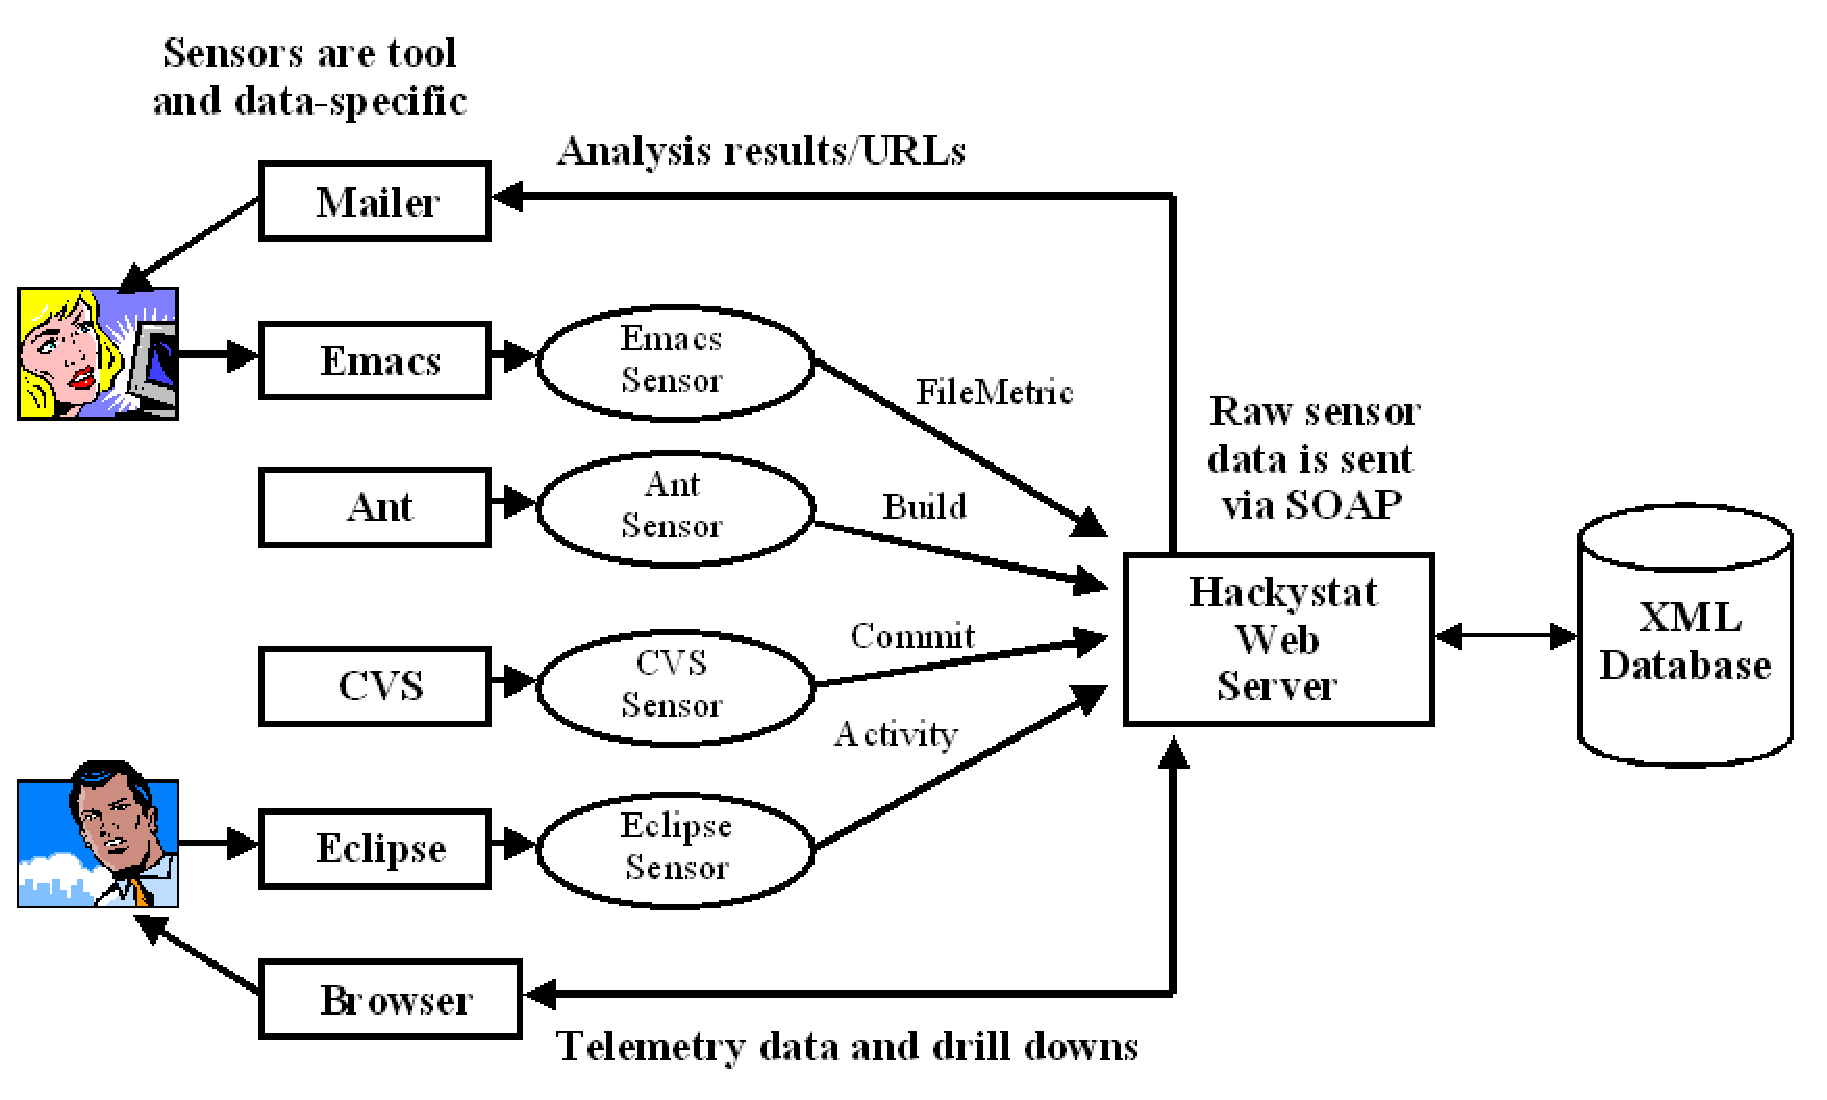
\includegraphics[width=0.60\textwidth]{architecture.eps}
  \caption{The basic architecture of Hackystat.}
  \label{fig:architecture}
\end{figure*}

To use Hackystat, the project development environment is instrumented by
installing Hackystat sensors, which developers attach to the various tools
such as their editor, build system, configuration management system, and so
forth. Once installed, the Hackystat sensors unobtrusively monitor
development activities and send process and product data to a centralized
web server.  If a user is working offline, sensor data is written to a
local log file to be sent when connectivity can be re-established.  Project
members can log in to the web server to see the collected raw data and run
analyses that integrate and abstract the raw sensor data streams into
telemetry.  Hackystat also allows project members to configure ``alerts``
that watch for specific conditions in the sensor data stream and send email
when these conditions occur. Figure \ref{fig:architecture} illustrates the
basic architecture of the system.

Hackystat is an open source project. Its sources, binaries, and
documentation are freely available online.  We also maintain a public
server running the latest release of the system at
http://hackystat.ics.hawaii.edu.  Hackystat has been under active
development for approximately five years, and currently consists of
approximately 2500 classes and 300,000 lines of code.  Sensors are available
for a variety of tools including Eclipse, Emacs, JBuilder, Jupiter, Jira,
Visual Studio, Ant, JUnit, JBlanket, CCCC, DependencyFinder, Harvest, LOCC,
Office, CVS, and SVN.

Hackystat is being used in a variety of academic and industrial contexts.
At the University of Hawaii, Hackystat has been  integrated into the
undergraduate and graduate software engineering curriculum, and is
used by approximately 50 students per year to support project
development \cite{csdl2-03-12}.  A researcher from the Free University of
Bozen came to Hawaii to study the Hackystat system in support their research on
PROM \cite{Sillitti03}.  Researchers at the University of Maryland are
using Hackystat to support assessment of programmer effort
\cite{Hochstein05}.  Hackystat has been used at NASA's Jet Propulsion
Lab to analyze the daily build process for the Mission Data System
\cite{csdl2-03-07}.  Finally, Hackystat is being used at SUN Microsystems
to support research on high performance computing system development
productivity \cite{csdl2-04-03}.

\subsection {Software Project Telemetry}
\label{sec:telemetry}

The automated, unobtrusive, continuous, and low-cost measurement
infrastructure provided by Hackystat enabled us to develop a new approach
to software measurement analysis called ``Software Project Telemetry``. 
According to Encyclopedia Brittanica, telemetry is a ``highly automated
communications process by which measurements are made and other data
collected at remote or inaccessible points and transmitted to receiving
equipment for monitoring, display, and recording.''  We
define Software Project Telemetry as a style of software engineering
process and product collection and analysis which satisfies the following
five properties:

{\em (1) Software project telemetry data is collected automatically by tools
that unobtrusively monitor some form of state in the project development
environment.}  In other words, the software developers are working in a
``remote or inaccessible location'' from the perspective of metrics
collection activities. This contrasts with software metrics data that
requires human intervention or developer effort to collect, such as PSP/TSP
metrics \cite{Humphrey95}.
        
{\em (2) Software project telemetry data consists of a stream of
time-stamped events, where the time-stamp is significant for analysis.}
Software project telemetry data is thus focused on evolutionary processes
in development.  This contrasts, for example, with COCOMO \cite{Boehm00},
where the moment in time at which calibration data is collected is not
generally significant.

{\em (3) Software project telemetry data is continuously and immediately
available to both developers and managers.}  Telemetry data is not hidden
away in some obscure database guarded by the software quality improvement
group.  It is easily visible to all members of the project for
interpretation.

{\em (4) Software project telemetry exhibits graceful degradation.}  While
complete telemetry data provides the best support for project management,
the analyses should not be brittle: they should still provide value even if
sensor data occasionally ``drops out`` during the project. Telemetry
collection and analysis should provide decision-making value even if these
activities start midway through a project.
         
{\em (5) Software project telemetry is used for in-process monitoring, control,
and short-term prediction.} Telemetry analyses provide representations of
current project state and how it is changing at the time scales of days,
weeks, or months.  The simultaneous display of multiple project state
values and how they change over the same time periods allow opportunistic
analyses---the emergent knowledge that one state variable appears to
co-vary with another in the context of the current project.

Software Project Telemetry enables an incremental, distributed,
visible, and experiential approach to project decision-making. For example,
if one finds that complexity telemetry values are increasing, {\em and}
that defect density telemetry values are also increasing, then one could
try corrective action (such as simplification of overly complex modules)
and see if that results in a decrease in defect density telemetry
values. One can also monitor other telemetry data to see if such
simplification has unintended side-effects (such as performance
degradation).  Project management using telemetry thus involves cycles of
hypothesis generation (Does module complexity correlate with defect
density?), hypothesis testing (If I reduce module complexity, then will
defect density decrease?), and impact analysis (Do the process changes
required to reduce module complexity produce unintended side-effects?).
Finally, Software Project Telemetry supports decentralized project
management: since telemetry data is visible to all members of the project,
it enables all members of the project--developers and managers--to engage
in these management activities.  

\begin{figure*}[ht]
  \centering
  \includegraphics[width=0.60\textwidth]{BuildAndChurn.eps}
  \caption{Telemetry illustrating how code churn co-varies with build failures.} 
  \label{fig:telemetryreport}
\end{figure*}

As a concrete example of telemetry, consider Figure
\ref{fig:telemetryreport}. This report illustrates the relationship between
aggregate code churn (the lines added and deleted from the CVS repository
by all members of the project) and the number of build failures
over a four month period on the Hackystat project. Note how closely these
two measures co-vary, even though one is a process measure (build failure)
and the other is a product measure (code churn).  From this initial
observation, one could investigate other time periods and time scales to
see if this relationship holds in other contexts, as well as test
hypotheses on how to reduce build failures or predict their impact on the
project schedule.

The computational path from the sensors in Figure \ref{fig:architecture} to
the telemetry report in Figure \ref{fig:telemetryreport} involves several
steps.  In the first step, ``raw'' sensor data is collected from small
software plug-ins attached to developer tools. For example, an editor
sensor may record a ``state change'' event when a file has been edited
within the last 30 seconds by the user.  A CVS sensor may record the number
of lines added and deleted from a file during the past 24 hours.  This raw
data is sent from the sensors to a Hackystat server, where they are
persisted in an XML-based repository.  In the second step, the system
abstracts the raw sensor data into one or more ``DailyProjectData''
instances, which synthesize raw sensor data from multiple group members
and/or multiple sensors into a higher level abstraction.  For example, a
DailyProjectData instance might process low-level ``state change'' events
from multiple developers and determine the total amount of time spent
editing files by all members of the project group for a given day.  In the
third step, special classes called ``Reduction Functions'' manipulate
DailyProjectData instances to create the sequence of numerical telemetry
values associated with a given project and time interval. For example, a
Reduction Function might manipulate a set of DailyProjectData instances to
produce a sequence of numerical telemetry values indicating LOC/hour.  In
the fourth step, the developer defines a Telemetry Chart or Report, which
specifies what types of product and process data should be displayed
together.  Finally, the Telemetry Chart or Report is instantiated for a
specific Project and time interval.

In one application of Software Project Telemetry, we are
creating telemetry streams to support diagnosis of daily build failures and
reduce the productivity impact of their occurrence over time
\cite{csdl2-04-11}.  Another application involves the development of
specialized telemetry streams for high performance computing software to
better understand the bottlenecks present in the development of those
systems \cite{csdl2-04-22}.

\subsection{Evidence-based software engineering}

A recent revolution in medical research involves the introduction of an
``evidence-based'' paradigm.  This paradigm arose in response to two
observations: the failure to organize medical research into systematic
reviews could cost lives, and the clinical judgement of experts compared
unfavorably with the results of systematic reviews.   The evidence-based 
approach is starting to be applied outside of medicine, in fields such as
psychiatry, nursing, social policy, education, and software engineering. 

Kitchenham has been leading the movement for evidence-based software
engineering, organizing workshops on this topic and publishing papers
explaining the issues involved in applying evidence-based research
techniques to software engineering \cite{Kitchenham04,Kitchenham04a}.  She
and her collaborators propose a five step method for evidence-based
software engineering: (1) Convert the need for information [about a
software engineering practice] into an answerable question; (2) Track down
the best evidence available for answering the question; (3) Critically
appraise that evidence using systematic review for its validity (closeness
to the truth), impact (size of the effect), and applicability (usefulness
in software development practice); (4) Integrate the critical appraisal
with current software engineering knowledge and stakeholder values [to
support decision-making]; (5) Evaluate the effectiveness and efficiency in
applying Steps 1-4 and seek ways to improve them for next time.  While
promising, application of systematic reviews and the integration of
empirical software engineering data from multiple sources has been found to
be challenging \cite{Jedlitschka04}.

\subsection{Software process research}

Osterweil has developed a view of software process research that recognizes
two complementary levels: macroprocess and microprocess \cite{Osterweil05}.
Macroprocess research is focused on the outward manifestations of
process---the time taken, costs incurred, defects generated, and so
forth. Macroprocess research traditionally correlates such outcome measures
to other project characteristics, which can suggest the impact of process
changes to these outcomes, but which suffers from the lack of any
underlying causal theory.  Bridging this gap is the province of
microprocess research, according to Osterweil, in which languages and
formal notations are used to specify process details at a sufficient level
of rigor and precision that they can be used to support causal explanation
of the outcome measures observed at the macroprocess level. In most cases,
these forms of software process research are ``top-down'', in that the goal
is to specify a ``best practice'' in abstract terms and in such a way that
it can be enforced within the development environment \cite{Shepard92,Jager99,DiNitto2002,Cass2000,Schlenoff00,Sutton97}.  
Our research most
readily fits into the ``microprocess'' level, except that instead of
specifying a top-down language, our approach focuses on bottom-up
recognition of the ``actual'' process. 

The Balboa research project, like our proposed research, is concerned with
bottom-up inference of process from low-level event streams \cite{Cook:95}. In
Balboa, the event streams are taken from the commit records of a
configuration management system, and finite state machines are created that
model the commit stream data observed in practice.  More recently, work has
been done on understanding processes associated with open source software
development processes \cite{Jensen:05}. In this research, ``web information
spaces'' are mined with the goal of discovering software process workflows
via analysis of their content, structure, update, and usage patterns. Our
approach.  Our proposed approach contrasts with these by employing sensor
instrumentation attached to a broad variety of developer tools including
their interactive development environment. This enables our analysis
mechanisms access to much lower-level events than those available through
the commit records of a configuration management system or through
web-based information sources.


\subsection{Results from prior NSF research}

\small
\begin{tabular}{lp{4.5in}}

Award number: & CCF02-34568 \\
Program: & Highly Dependable Computing and Communication Systems Research\\
Amount: & \$638,000 \\
Period of support: & September 2002 to September 2007 \\
Title of Project: & Supporting development of highly dependable software through
continuous, automated, in-process, and individualized software measurement validation \\
Principal Investigator: & Philip M. Johnson \\
Selected Publications: & \cite{csdl2-04-22,csdl2-04-13,csdl2-04-11,csdl2-03-12,
csdl2-02-07,csdl2-03-07,csdl2-04-02,csdl2-04-04,csdl2-04-06}
\end{tabular} \\ %[3mm]
\normalsize

\medskip

The general objective of this  research project is to design,
implement, and validate software measures within a development
infrastructure that supports the development of highly dependable software
systems.  Contributions of this research project include: (a) development
of a specialized configuration of Hackystat to automatically acquire build
and workflow data from the configuration management system for the Mission
Data System (MDS) project at Jet Propulsion Laboratory; (b) development of
analyses over MDS build and workflow data to support identification of
potential bottlenecks and process validation; (c) identification of
previous unknown variation within the MDS development process; (d)
development of a generalized approach to in-process, continuous measurement
validation called Software Project Telemetry, (e) substantial enhancements
to the open source Hackystat framework, improving its generality and
usability; (f) development of undergraduate and graduate software
engineering curriculum involving the use of Hackystat for automated
software engineering metrics collection and analysis; (g) support for 3
Ph.D., 6 M.S., and 3 B.S. degree students.

\section{Research Plan}
\label{sec:research-plan}

To evaluate the feasibility of this research approach, we have already implemented
a prototype version of SDSA, augmented it with rules for the Test Driven
Development best practice, and performed a pre-pilot study on a small set
of students.  These preliminary results are encouraging and suggest that
SDSA does have the potential to recognize at least one non-trivial software
engineering best practice.  However, significant research questions remain:
will these preliminary results hold up when applied to more sophisticated
users of TDD?  What are effective approaches to validation of the
recognition rules?  What are the limitations of the Hackystat sensor-based
technology for gathering the raw data necessary for best practice
recognition?  Can SDSA still be useful when only ``partial'' recognition is
possible?  Can our prototype single user version of SDSA scale to
recognition of behavioral patterns across groups of developers? Finally,
what is the most effective way to design, package, and distribute the
technology to support replication, adoption, and enhancement to support new
practices by other organizations?

To provide insight into these research questions and our research task, the
next section provides more details on our proposed analysis mechanism.

\subsection{Software Development Stream Analysis}

Software Project Telemetry supports a ``macro'' view of project
development: telemetry aggregates process and product data gathered by the
developers in a project and how they change at time scales of days, weeks,
or months.  In contrast, our proposed Software Development Stream Analysis
mechanism focuses on a ``micro'' view of project development, which seeks
to analyze the behaviors of a single developer at the time scale of minutes
or hours and characterize the practices, if any, being employed by the
developer.

To make this concrete, consider the best practice called ``test driven
design'' (TDD) \cite{Beck03}.  TDD is often explained through a stop light
metaphor, which cycles from green to yellow to red.  At the beginning of a
TDD cycle, the code is working, and the stop light is green.  The developer
then defines a new test case that tests a new (and as yet unimplemented)
feature.  This will produce a syntax (compilation) error because that
feature is not even implemented yet.  This changes the stop light to
yellow.  Consequently, the developer implements a stub version of the
feature, which fixes the compilation error but produces a test failure.
This changes the stop light to red. Once the developer finishes
implementing the feature, the light changes to green and the cycle begins
again.  The stop light metaphor is interesting because out of sequence
lights indicate violations of the TDD development pattern; for example,
green to red indicates that the developer added new code without adding a
test for it first.

Recognizing practices such as TDD using SDSA involves a multi-step
process. First, Hackystat sensors collect raw data sufficient to allow
identification of the development behavior of interest. In the case of a
practice like TDD, only a sensor for the IDE is required, and it collects
editing events, compilation events, refactoring events, and test invocation
events.  These events are sent to the Hackystat server for further
analysis.  On the server side, the second step
involves ``tokenization'', which essentially replaces sequences of raw data
representing the same type of behavior by a single token representing that
behavior. For example, if the user edits the same file for several minutes,
several dozen editing events may be generated in the raw data stream. The
SDSA tokenizer replaces these by a single ``Edit'' token. Third, SDSA
applies rules for partitioning the single tokenized event stream into a
sequence of ``episodes'', where each episode represents a behavioral
sequence that can be recognized as belonging to the practice or not.  In
the case of the TDD best practice, an appropriate episode boundary is when
all of the unit tests pass.  Fourth, SDSA applies classification rules based 
upon the open source JESS framework \cite{Friedman-Hill:03} to
identify each episode as belonging to the best practice or not.  For
example, an episode belonging to the TDD practice might consists of a
sequence of tokens indicating: (a) creation of a test case; (b) a failed
attempt to compile the test case; (c) editing (presumably to fix the
compilation error by implementing the production code invoked in the test
case); (d) invocation and failure of the test case (presumably due to a bug
in the implementation); (e) further editing; and (f) successful test case
invocation (which also signals the episode boundary).

This all sounds good in theory, but does it actually work in practice?  Can
sensors actually capture the raw data necessary for higher-level analyses? 
Can appropriate episode boundaries be defined? Finally, does the model of 
the best practice as defined by the recognition rules correspond to the 
reality of the best practice as understood by practitioners? 

To provide an initial feasibility check of SDSA, we performed a pre-pilot
study \cite{csdl2-06-02}. For this study, we created a package called Zorro
that extends the generic SDSA mechanism with the episode recognition and
classification rules for TDD.  We also implemented a system called
``Eclipse Screen Recorder'' (ESR), which creates a QuickTime movie of the
Eclipse window.  We then asked seven volunteers to develop a simple
application in Eclipse while following basic Test Driven Design practices.
The participants completed the task in a single programming session that
typically lasted between 30 and 60 minutes. We captured their development
behaviors in two independent ways: through the sensor events collected by
Hackystat as well as though the QuickTime movie created using ESR.  Using
the QuickTime movie, we performed a validation of the Zorro TDD recognition
package, checking that the movie of developer behaviors corresponded to the
behavioral patterns inferred by Zorro.  Our results revealed opportunities
for improvement in both sensor data collection and rule definition, but
despite these problems we found that Zorro correctly classified 89\% of the
92 episodes generated in this study.

The success of our pre-pilot study gives us confidence that SDSA is a
viable research direction and reduces some of the risk factors associated
with this project.

\subsection{Task descriptions}

Our research plan follows the detailed objectives for this research as
summarized in Section \ref{sec:objectives}, and consists of the following tasks.

{\bf (1) Enhance the Software Development Stream Analysis mechanism.} 
There are two primary kinds of enhancements that we propose in this research.
The first involves more sophisticated support for validation.   In our pre-pilot 
research, we used the Eclipse Screen Recorder to obtain an independent view of 
developer behaviors.  One limitation of this technique is that it relies on the
experimenters own definition of TDD.  To overcome this limitation, we would like to provide
users with the ability to review and confirm the inferences made by the system, 
which can provide valuable feedback about the practice as understood by the 
practitioners themselves.  

\begin{figure*}[ht]
  \centering
  \includegraphics[width=0.90\textwidth]{zorro-interface.eps}
  \caption{A mockup of an enhanced SDSA validation interface.}
  \label{fig:zorro}
\end{figure*}

Figure \ref{fig:zorro} illustrates a mockup of an interface for TDD
validation.  Each row in this interface represents an episode.  The
interface allows the user to provide feedback about the classification of
each episode after review of the classification made and the reasons behind
it (which are automatically generated by traversing the rule base).

A second task associated with this objective is to expand the range of practices
supported by SDSA in order to better understand its strengths and limitations. 
We intend to expand support for agile programming practices beyond TDD to 
pair programming and continuous integration. 

In addition, we plan to extend SDSA to support high performance computing
best practices, based upon our association with the DARPA High Productivity
Computing Systems (HPCS) program.  One of the workflow models identified in
this program separates high performance computing development activities
into serial coding, parallel coding, debugging, and optimization. However,
there is debate within the community regarding the way these workflow
activities should be organized: some advocate serial coding first (in order
to establish functional correctness without the complexity of
parallelization), while others advocate parallel coding first (to establish
a parallel framework within which to embed the serial code).  There is even
debate as to whether this workflow decomposition is the appropriate way to
characterize HPC development.  Research on an SDSA-based recognition
mechanism for HPC activities can both provide empirical data regarding
these debates, as well as help us understand the strengths and limitations
of the SDSA approach.

{\bf (2) Develop integration mechanisms between SDSA and Software
Project Telemetry.}  Currently, Hackystat does not provide any support for
relating the analyses of SDSA to those of Software Project Telemetry.  In
this task, we will develop such mechanisms.  In general, the goal is to
support the display of relationships in two directions. Given the
identification of an interesting SDSA behavior, we will display
potentially relevant telemetry streams in the period surrounding that
behavior.  Conversely, given the identification of an interesting change in
the telemetry associated with a given project, we will display the
SDSA behaviors in the period surrounding that change.  

We have already found that in some cases, it is possible to convert the
SDSA results into telemetry streams, greatly simplifying the
integration. For example, the Zorro system provides a telemetry stream
representing the percentage of episodes during the day recognized as
TDD-compliant. This makes a number of interesting telemetry-based analyses
easily available, such as one that shows how test case coverage varies with
the percentage of TDD-compliant episodes during development over time.
Given that TDD is purported to achieve 100\% test coverage as a natural
by-product of the practice, this telemetry can help verify that claim, and
also see if ``graceful degradation'' in coverage levels occurs if the percentage
of TDD-compliant episodes goes below 100\%.

{\bf (3) Perform classroom-based, case study evaluation of the proposed
techniques.}  Once we have implementations of SDSA and its Telemetry
integration, we will perform studies to assess their utility and
effectiveness in classroom conditions.  Over the past several years, we
have integrated Hackystat into the undergraduate and graduate software
engineering curriculum at the University of Hawaii. Our students now
routinely install sensors, collect and analyze process and product metrics,
and use this data to guide project management \cite{csdl2-03-12}.  This
provides an excellent environment for initial evaluation of new Hackystat-based
technologies.

We plan to evaluate SDSA and Telemetry integration though a case study of
test-driven design with three experimental phases.  In the first phase at
the beginning of the course, we will introduce ``traditional'' unit testing
and have them carry out a project assignment that requires them to achieve
at least 90\% coverage (to guarantee a minimal level of test case quality)
but without specifying when or how to develop the test cases.  We will use
SDSA to verify that students are not using TDD for this phase, and use
Software Telemetry to assess coverage, LOC/Hour, and other indicators of
quality and productivity.

In the second phase of the experiment, we will introduce principles of TDD,
provide a short assignment for them to use to learn TDD, then have them
carry out a project assignment that requires both the use of TDD and at
least 90\% coverage.We will use SDSA to verify that the students are using
TDD during this project, and Software Telemetry to assess the same
indicators of quality and productivity as before.  We can compare the
values of these indicators to see if any changes occur from the
introduction of TDD. For example, does the introduction of the TDD best
practice improve average programming productivity?  Does it decrease the
variation in programmer productivity?  Finally, we will use validation facilities 
like the mockup illustrated in Figure \ref{fig:zorro} to obtain developer opinions
on classification accuracy. 

In the third phase of the experiment, we will have the students carry out a
final project assignment, and this time require 90\% coverage but allow
them to choose their test development process.  We will use SDSA to
determine what percentage of the students use TDD and how consistently they
use TDD. We will use telemetry to see how quality and productivity measures
have changed relative to earlier phases.

At the end of the study, we will collect qualitative data using a questionnaire to
assess student attitudes towards Hackystat, TDD, and SDSA.

We foresee multiple uses for the results from this case study.  First, it
will provide useful information about the robustness and utility of our
technology. For example, can SDSA correctly characterize developer behavior
as TDD, and to what extent is it susceptible to false positives and false
negatives? In addition, the case study data can yield interesting empirical
evidence regarding the efficacy of TDD, its impact on programmer
productivity and variability, and provide an empirical, replicable test of
the claims made by its proponents.

{\bf (4) Perform industry-based evaluation of SDSA and Telemetry.}  Once our
classroom evaluation is under way and we feel confident that the technology
and methods are sound, we plan to carry out two industrial case studies.

The first industry case study will involve programmers affiliated with the
DARPA High Productivity Computing Systems program.  In this case study, we
will identify a high performance system software development group
interested in obtaining empirical data regarding their HPC development
practices, install the enhancements described above in (1), monitor usage,
and collect validation data to assess the accuracy of the inferences.  We
anticipate that the size of this development group will be on the order of
6-10 developers, and that we will monitor their practices over a period of
approximately six months.

The second industry case study will use SDSA to assess test-driven
development in an industrial setting.  We will publish a call for an ``open
evaluation'' of agile practices at such conferences as XP/Agile Universe
and internet sites such as the Agile Alliance.  We hope to attract
approximately 50 participants who will agree to have their agile
development practices monitored for a period of one week. Participants will
download and install the appropriate sensors and begin sending data to the
Hackystat public server.  We will use the enhanced version of SDSA as
discussed above to determine when they are performing agile activities such
as TDD, pair programming, and continuous integration.  The server will
provide them with analyses of their data, and include validation mechanisms
to enable them to report on the correctness of the classification
mechanisms.  At the conclusion of the open evaluation, we will distribute a
questionnaire to participants to collect data on their experience and
demographic information that we can use to better understand the context in
which their data was generated.

The industrial case study results will be used to assess the robustness and
utility of the Telemetry and SDSA mechanisms outside of a controlled
classroom setting. In addition, the case studies will produce new empirical
evidence regarding TDD and HPC best practices.  Finally, it will provide
insights into the limitations of this research approach, including (a) the
extent to which automated sensor-based technology and rule-based inference
is adequate to recognize best practices in industrial settings, and (b) the
privacy and organizational barriers to successful adoption of this
approach.

{\bf (5) Package the system and methods for widespread dissemination.} 
Our approach to this task is highly influenced by the movement toward
evidence-based software engineering, which seeks the introduction of
systematic reviews to improve the quality of our understanding of
practices, the increased use of replication to better understand the
context surrounding empirical results, and a better understanding of how 
evidence can be used to support the practice of software engineering in 
real world contexts.   

As Hackystat and its associated applications are open source software with
a well-developed infrastructure for distributed development, the packaging
of the actual software for widespread dissemination is straightforward.  A
more challenging problem is to package the experimental methods such that
the software can be used effectively to produce empirical evidence that
adds new value to a systematic review of the literature, either via
replication of an existing experiment or via a modification to an existing
method.  We plan to build upon prior research by Basili and his colleagues
on ``Experience Factories'' \cite{Basili94} to create ``kits'' combining a
Hackystat software configuration with documentation detailing the sensors
to install, the data to collect, and the analyses to perform to gain
insight into the best practice of interest.

{\bf (6) Develop curriculum materials.}  Our prior experience with
Hackystat in the classroom setting convinces us that collection and
analysis of software engineering metrics can form a compelling motivation
for the use of software engineering practices such as unit testing,
configuration management, and software review.  For this task, we will
incorporate the technology and methods from this evidence-based approach to
best practices into our undergraduate and graduate software engineering
curriculum.  We will teach the theory of evidence-based software
engineering, show data from prior studies and discuss its implications, and
most importantly, enable students to experience the gathering and analysis
of evidence about their own practice through the use of Hackystat, SDSA,
and Software Project Telemetry on classroom projects.

\subsection{Work breakdown structure and milestones}

\begin{figure*}[ht]
  \centering
  \includegraphics[width=0.75\textwidth]{workstructure.eps}
  \caption{Work breakdown structure and milestones.} 
  \label{fig:wbs}
\end{figure*}


Figure \ref{fig:wbs} shows when we plan to carry out each of these
tasks, along with three milestones.  As illustrated, we will be
working on SDSA enhancement for almost the entire time of the project.  The case studies 
will begin in year two, and the packaging and curriculum material generation will be the primary
focus of year three. We also plan for three major
milestones during the project, occurring near the end of each of the three
years of the research. The milestones are denoted by upcoming major
releases of the Hackystat framework and its associated applications.
Release 8.0 will include the enhanced software development stream analysis
mechanism, along with integration mechanisms for software project
telemetry.  Release 9.0 will incorporate enhancements based upon the classroom studies. 
At the end of the project, we will release 10.0, which enhances the prior
releases with the all of the results from the project. 

It is also important to identify and manage the risk factors associated
with this research plan.  We view the enhancement of SDSA as having
moderate risk, in that we do not yet know how well the current SDSA design
generalizes beyond the case of test-driven design.  It may be that
substantial redesign will be required to generalize our approach to best
practice representation beyond TDD.  The SDSA/Telemetry integration task
has low risk: this is an engineering modification to the Hackystat
framework that we are well suited to accomplishing.  The classroom case
studies have low risk: we have a great deal of experience with classroom
case studies and have ready access to the software engineering student
population at the University of Hawaii.  The industry case studies have
moderate risk; while we have an excellent collaborative relationship with
the DARPA HPCS participants, there are always political and organizational hurdles to
cross before a case study can occur on a real-world project.  The TDD case
studies include the risk of failing to attract interest from the Agile
development community.  Finally, the packaging, dissemination, and
curriculum material development tasks have low risk; we have been
developing curriculum materials and packaging/disseminating our Hackystat
research for a number of years and are experienced with this activity.

\section{Conclusions}

In all fields of human endeavor, there are extraordinarily gifted
practitioners: in music, Beethoven and Mozart; in golf, Wie and
Woods; in software development, Stallman and Joy.  While no technological
innovation can match innate genius, the ultimate goal of this research is
to provide the tools and techniques to allow all software developers to
reach their maximal potential.

Our proposal presents research designed to produce a variety of
contributions to the theory and practice of software engineering as well as
broader impact to society at large.  First, it will yield new technological
infrastructure for continuously collecting, analyzing, and interpreting software
engineering best practices.  This infrastructure will be novel in its
ability to collect and analyze both ``macro'' level project characteristics
and ``micro'' level developer practices and relate these two levels of
information to each other.  

Second, the research will yield a set of case studies in both classroom and
industrial settings.  The studies are designed to provide new empirical
data about software engineering, new insights into how best practices and
be represented and used, and specific data about programmer productivity
and behavior in domains including  high performance computing and 
agile development.  It will also provide findings regarding the limitations of
this approach due to technical or organizational factors. 

Third, the research is grounded in an evidence-based approach to software
engineering, which should yield results more easily available to systematic
review, replication, and enhancement.  We intend for our curriculum
materials to be leveraged by other teachers and result in improved use of
metrics in software engineering practice.  As the University of Hawaii is a
university with 75\% minority students in an EPSCOR state, this research
will provide novel research opportunities to underrepresented groups.

There was a sign that hung in Albert Einstein's office at Princeton
University: ``Not everything that counts can be counted, and not everything
that can be counted counts''.  This cautionary statement is certainly
relevent to our proposed research.  However, we believe that this
combination of contributions, if successful, will provide one more step
toward safer, sounder, and more cost-effective information technology for
our society.










